% !TeX root = ../main.tex
% Add the above to each chapter to make compiling the PDF easier in some editors.

\chapter{Introduction}\label{chapter:introduction}

This chapter explains the problem we are addressing, why, a brief overview of our solution, and the attacks we are trying to fend off.

% nicht wissenschaftliche Teil, zero trust ist jetzt ein Ding, immer mehr embedded ohne TPM (z.B. Gartner Studien)

\section{Motivation}

% Which area this thesis is talking about (Zero Trust)

Modern trust relationships, such as Zero Trust~\cite{isaca2021}, require trustworthy platforms to reliably report their system state.
In such models, trust is no longer implicitly assumed, e.g., by the fact that a device is located within the boundaries of a company.
Instead, each device is considered compromised until proven otherwise on a per-request basis for resources (e.g., printers) and data access~\cite{Rose2020}.

% Primer on remote attestation

This is solved by remote attestation.
In the simplest case, there is a prover and a verifier, as depicted in \autoref{fig:ra_simple}.
The challenge is that the verifier observes nothing but bytes from the prover, and while a benign prover will tell the truth about its state, a compromised prover will lie about its state and claim a trustworthy one.
Therefore, the verifier must establish trust in a helper component on the prover's side.
In a typical setup, this component is immutable without the involvement of its manufacturer, which reveals itself to a verifier by signing and storing a certificate on the helper components supplied by it.
This allows the verifier to establish trust in the helper component by knowing its manufacturer.
Consequently, the component attests to the state of the prover's machine, from which the verifier can deduce whether the prover can be considered trustworthy.

\begin{figure}[htpb]
  \centering
  \includegraphics[width=0.5\linewidth]{figures/remote_attestation_process.pdf}
  \caption{Simplified remote attestation process.}\label{fig:ra_simple}
\end{figure}


% TPMs become more important

For example, this can be done with a \ac{TPM} on the prover's side. They rise in their deployments and importance, e.g., in 2013, the President's Council of Advisors on Science and Technology encouraged the adoption of TPMs~\cite{usa}, and Microsoft publicized that they require a TPM module for Windows~11 in 2021~\cite{win11req}.
They provide remote attestation mechanisms of system states, and their applications are still expanding beyond their traditional use cases. For example, they are used in anti-cheat software for games~\cite{valorant}.

% Short intro on why fTPMs were introduced (for weak devices, exactly our target platform)

A \ac{dTPM} increases cost and hardware complexity---especially for embedded platforms.
\Acp{fTPM} running in a \acp{TEE} can be used to provide similar security guarantees as a \ac{dTPM} chip.

% Why establishing trust in an fTPM is harder than in a dTPM

For a \ac{dTPM}, which consists of an independent hardware unit manufactured by a single manufacturer, it is sufficient to identify its manufacturer and understand their provided guarantees.
In contrast, an \ac{fTPM} runs atop other firmware components and is started later in the boot chain, making its security dependent on the underlying firmware stack.
Consequently, trust in an \ac{fTPM} depends on trusting the entire stack beneath it because its underlying firmware might alter or compromise the \ac{fTPM}.

% What's the difficulty of establishing trust in an fTPM?

However, while a TPM-compliant component provides an infrastructure with which trust in it can be established remotely, i.e., an endorsement (key) certificate~(EKcert), this does not represent the underlying firmware stack.

% How it currently works for fTPMs

Currently, this is solved by the manufacturer providing not only the fTPM, but also the entire underlying firmware stack.
Consequently, by establishing trust in the manufacturer of the fTPM, one can implicitly trust the underlying firmware by assuming they also originate from this manufacturer.
This is possible since, in the most general sense, one can derive from an endorsement certificate the endorser, i.e., manufacturer.
If the attester trusts the manufacturer and its provided guarantees, trust is established in its provided components.

\begin{figure}[htpb]
  \centering
  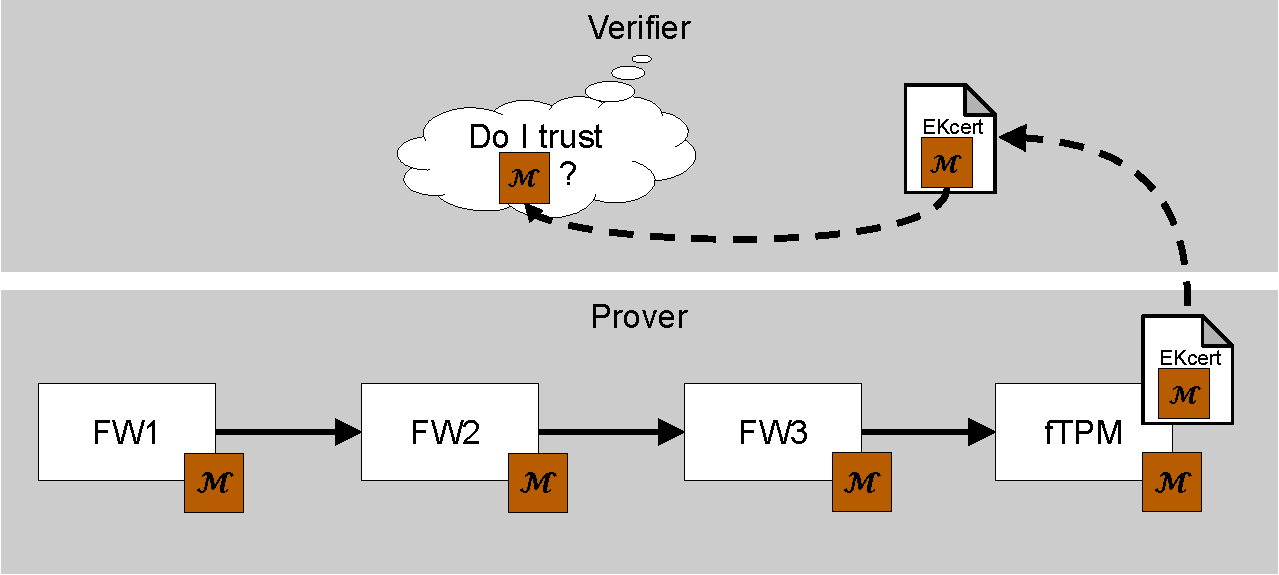
\includegraphics[width=1\linewidth]{figures/current_state.pdf}
  \caption{The naive process how a verifier establishes trust to an \ac{fTPM}, which is in fact done by trusting its manufacturer. The brown markers indicate a manufacturer. The firmware~(FW) and the fTPM were built by manufacturer \(\mathcal{M}\), and the EK certificate indicates this manufacturer.}\label{fig:current_state}
\end{figure}


This process is illustrated in figure \autoref{fig:current_state}.
The prover's box shows its boot chain, and the verifier's box shows how it evaluates the trustworthiness against the prover's boot chain.
The verifier trusts the entire firmware chain if it trusts the manufacturer of each component.
Note how the verifier must assume that the manufacturer of the firmware components is the same as that of the fTPM\@.
To the best of our knowledge, this is what manufacturers like Intel and AMD implement for their \acp{fTPM}, as confidence in their \acp{fTPM} is also only established through an EKcert~\cite{Ruan2014}.

% Summary with limitations

In summary, with the current approach, the endorser, usually a CPU manufacturer, provides the firmware up to the fTPM and guarantees the firmware is not modifiable by untrusted parties.
This enables trust in the other firmware components this manufacturer provided without knowing the firmware.
This approach is limited, as with this mechanism, independent verifiers have to unquestioningly trust the firmware manufacturer, drastically limiting trust relationships.

\section{Goal}

We establish an independently verifiable fTPM stack, rooted in a hardware root of trust, that can be leveraged in a Zero Trust environment with few hardware requirements and without compromising security.
This approach aims to break the requirement of the underlying firmware and the fTPM to originate from the same manufacturer by providing the exact firmware component identities to the verifier, such that it can decide whether they are trustworthy without relying on its manufacturer.
Instead, it is sufficient to trust the independent manufacturer of the hardware root of trust, which requires minimal assumptions, such as the absence of side-channel vulnerabilities.

% Short introduction to DICE

One mechanism enabling firmware attestation is the \ac{DICE}, focusing on resource-constrained devices.
Although this mechanism shifts trust from the firmware provider to the hardware provider by allowing firmware attestation through a hardware root of trust, the exclusive use of this integrated solution is unsuitable for large dynamic systems, such as Linux-based devices.
Nevertheless, the advantage is that the identity of each component of the firmware boot chain is represented.

% How we try to overcome these limitations

We propose a hybrid solution, combining the advantages of \ac{DICE} and \acp{fTPM}, yielding an independently verifiable certificate chain representing the boot chain up to and including the \ac{fTPM}.
This enables a verifier to establish trust in an \ac{fTPM} if the underlying firmware is also benign, thus providing a way to independently assess the properties of the \ac{fTPM}.
% The conceptual basis for this is to attest to the software stack of the TPM itself, thus providing a way to assess the properties of the fTPM independently.

%Current \ac{fTPM} implementations require additional security measures to not leak state between reboots and different software versions.
%The final concept should provide comprehensive guidelines for implementing an fTPM, which accounts for such an environment and reflects any relevant information through remote attestation.

The research questions we aim to answer are listed below.
\begin{enumerate}[label=\textbf{RQ-\arabic*}]
  \item What constitutes the identity of an fTPM\@?\label{rq:1-tpm-identity} %(e.g., hash, configuration, boot chain)
  \item How to combine the DICE and TPM infrastructure?\label{rq:2-combine-infrastructure} %(e.g., AliasCert $\cup$ EKcert)
  \item How to manage an fTPM's persistent data securely?\label{rq:3-secure-data} %(e.g., flush data on update)
  \item How to enable privacy in this attestation mechanism for the prover?\label{rq:4-privacy}
\end{enumerate}

% Prover and verifier can take both roles for mutual attestation

% Chaining the underlying firmware identities with the endorsement identity

\section{Threat Model}

% https://trustedfirmware-a.readthedocs.io/en/latest/threat_model/threat_model.html

% Attacker model: What an attacker can do (abilities) and cannot do (limits)

The attacker we are interested in can replace the fTPM or one of its predecessor components.
Therefore, there is a risk that a remote party trusts a firmware TPM that is not trustworthy.
For example, an attacker could install a malicious update of a relevant firmware component on the target device.
However, we assume the attacker can only do this before or during the device's boot process but not afterward.
Hardware, side-channel, control-flow, and denial-of-service attacks are out-of-scope.

For the network, we assume the Dolev-Yao attacker model~\cite{Dolev1983}, wherein an attacker can perform any active or passive attack on the network.
The attacker may also control parts or the entire network, e.g., all routers, switches, and connections.
Last, they cannot break cryptographic primitives, e.g., encryption, signing, and hashing.

\section{Security goals}

In this section, we want to formally describe the security goals of our solution so that we can later briefly discuss whether and how we achieve the corresponding objectives.

\begin{enumerate}[label=\textbf{SG-\arabic*}]
  \item{\textbf{Compromised fTPM cannot fake its identity}\\
  It is sufficient for a fake identity to be recognized by the verifier, who can consequently classify the prover's fTPM as untrustworthy.}\label{sg:1}
  % Does not have access to OP-TEE's private key; code in user mode does not have access to data in kernel mode

  \item{\textbf{Small root of trust}\\
  A small root of trust, e.g., in code size, hardware size, and complexity, bears less risk in implementation errors, directly affecting security~\cite{Singaravelu2006}.
  % and complexity, and its approaches to guarantee specific security properties are more manageable.
  }\label{sg:2}
  % DICE, its design, not concrete HW, its protection of the \ac{UDS}
  
  \item{\textbf{Isolation of fTPM storage}\\
  Data must only be accessible or modifiable within the boundaries of the fTPM's access controls, i.e., the TPM commands defined by its specification~\cite{tpm20}.
  This includes protecting against other trusted applications running in the same \ac{TEE}\@.}\label{sg:3}
  
  \item{\textbf{Protect fTPM data against downgrade attacks on the fTPM}\\
  Data of the fTPM should be sealed to its identity, such that when the fTPM is modified, e.g., by a downgrade attack, even the fTPM cannot access its old data anymore.}\label{sg:4}

  % \item{\textbf{Privacy of remote attestation process}\\
  % The verifier should be able to establish trust in an fTPM without having to know the identity of the fTPM, i.e., its EK\@.}\label{sg:5}
\end{enumerate}

\section{Outline}

In the \nameref{chapter:background}, we provide the knowledge necessary for a better understanding of the subsequent parts of this thesis.
Afterward, we discuss \nameref{chapter:related_work}, i.e., attacks on TPMs to further motivate this work, approaches to hardening TPMs, and work that enables remote attestation similar to ours.
Under \nameref{chapter:methodology}, we explain the concept of our solution and subsequently present our proof-of-concept \nameref{chapter:implementation}.
Finally, we \hyperref[chapter:discussion]{discuss} our design and implementation, rounded off by the \nameref{chapter:future_work_and_conclusion}.
